\documentclass{article}

\usepackage{graphicx}
\usepackage{float}
\usepackage{listings}
\usepackage{lstautogobble}
\usepackage{xepersian}

\graphicspath{{./img}}
\settextfont{XB Niloofar}

\title{سیستم‌های عامل - دکتر ابراهیمی‌مقدم}
\author{امیرحسین منصوری - ۹۹۲۴۳۰۶۹}
\date{تمرین سری اول}

\begin{document}
	\maketitle

	\section*{سوال ۱}
	\paragraph*{الف)}
	جمله درست است.

	\paragraph*{ب)}
	نادرست؛
	\textit{سیاست}
	(یا
	\lr{Policy})
	مشخص می‌کند که چه کاری انجام شود.
	\textit{مکانیزم}
	نحوه انجام کار را مشخص می‌کند.

	\paragraph*{پ)}
	نادرست؛ در
	\lr{Asymmetric Multiprocessing}،
	حافظه مشترکی وجود ندارد.

	\paragraph*{ت)}
	نادرست؛ اگر تعداد پارامترها زیاد باشد (بیشتر از تعداد رجیسترهای موجود)، پارامترهای دیگر را در مکانی در حافظه قرار می‌دهیم (مثلا پشته سیستم عامل)، و آدرس آن مکان از حافظه را در به عنوان پارامتر در یک رجیستر قرار می‌دهیم.

	\paragraph*{ث)}
	نادرست؛ سرویس‌های حیاتی‌تر مانند مدیریت حافظه یا
	\lr{CPU Scheduler}
	می‌توانند همچنان در هسته قرار بگیرند؛ هرچند که روی این موضوع که دقیقا چه سرویس‌هایی داخل کرنل اجرا می‌شود و چه سرویس‌های بیرون از آن، اتفاق نظر وجود ندارد.

	\section*{سوال ۲}

	\paragraph*{الف)}
	کاربرد اصلی آن، جلوگیری از اختلال در اجرای برنامه‌های دیگر، یا اجرای خود سیستم‌عامل، توسط یک برنامه مخرب یا نادرست است.

	\paragraph*{ب)}
	هنگام اجرای یک برنامه کاربری
	(\lr{User Program})
	و هر زمان که یک
	\lr{System Call}
	یا وقفه رخ می‌دهد، با تنظیم
	\lr{mode bit}
	به
	\lr{Kernel Mode}
	می‌رویم و کدهای سیستم‌عامل در این حالت اجرا می‌شوند.
	پس از اتمام کار سیستم‌عامل، دوباره با تنظیم
	\lr{mode bit}،
	به
	\lr{User Mode}
	می‌رویم و اجرای برنامه‌های کاربری ادامه پیدا می‌کنند.

	\paragraph*{پ)}
	این دو حالت عبارت‌اند از
	\lr{Kernel Mode}
	و
	\lr{User Mode}.
	تفاوت بین آن‌ها به صورت زیر است:

	\begin{enumerate}
		\item
		در حالت
		\LRE{Kernel mode}،
		بیشترین سطح دسترسی وجود دارد؛ به طوری که اجازه دسترسی مستقیم به سخت‌افزار نیز وجود دارد. اما در حالت
		\LRE{User mode}،
		دسترسی برنامه در حال اجرا توسط سیستم‌عامل کنترل می‌شود و دسترسی به سخت‌افزار تنها از راه صدازدن سیستم‌کال‌های سیستم‌عامل ممکن است.

		\item
		تغییر حالت از
		\LRE{Kernel mode}
		به
		\LRE{User mode}
		همیشه ممکن است، اما برعکس آن همیشه امکان‌پذیر نیست.

		\item
		در
		\LRE{Kernel mode}
		فضای آدرس‌دهی برنامه با هسته سیستم‌عامل مشترک است؛ ولی برای برنامه‌های
		\LRE{User mode}
		از حافظه مجازی
		(\LRE{Virtual Memory})
		استفاده می‌شود.
	\end{enumerate}

	\section*{سوال ۳}

	\paragraph*{الف)}
	وقفه یا
	\lr{Interrupt}
	روشی برای اطلاع دادن به پردازنده درباره یک رویداد است، که باعث توقف عملکرد عادی پردازنده و اجرای یک کد خاص برای پاسخ به این رویداد می‌شود. مثلا هنگام انجام یک عملیات ورودی/خروجی توسط پردازنده، که معمولا زمان‌بر است، پردازنده با اعمال یک وقفه سخت‌افزاری توسط ماژول ورودی/خروجی از اتمام عملیات آگاه می‌شود و می‌تواند نتیجه عملیات را بخواند و روی آن پردازش انجام دهد. به این ترتیب، پردازنده نیاز به صبر کردن برای اتمام کارهای زمان‌بر (مثلا عملیات ورودی/خروجی) ندارد و می‌تواند در این حین، کارهای دیگر را انجام دهد.
	\paragraph*{}
	وقفه می‌تواند سخت‌افزاری یا نرم‌افزاری باشد. همچنین می‌توان برای هر رویداد یک وقفه جداگانه تعریف کرد و به آن یک شماره خاص اختصاص داد. همچنین می‌توان برخی وقفه‌ها را
	\lr{mask}
	کرد؛ به این ترتیب، این وقفه‌ها نادیده گرفته می‌شوند و در صورت آمدن آن‌ها، تاثیری در عملکرد پردازنده نخواهند داشت. برای وقفه‌ها نیز می‌توان
	\textit{اولویت}
	در نظر گرفت، تا در صورت آمدن همزمان چندین وقفه بتوان درباره پذیرش آن‌ها تصمیم‌گیری کرد.

	\paragraph*{ب)}
	سرکشی یا
	\lr{Polling}
	روش دیگری برای بررسی رویدادهای خارجی (مثل عملیات ورودی/خروجی) است. در این روش، یک کد نرم‌افزاری رخ دادن رویداد را به طور مداوم بررسی می‌کند و به این ترتیب، تا زمان رخ‌دادن آن صبر می‌کند و سپس به ادامه کار عادی خود می‌پردازد.

	\paragraph*{}
	این روش، برای زمانی که بخواهیم با سرعت زیاد رویدادهای خارجی را پردازش کنیم مناسب نیست و سربار بالایی دارد.

	\paragraph*{پ)}
	بردار وقفه یا
	\lr{Interrupt Vector}
	جدولی شامل آدرس مربوط به ابتدای کد
	\lr{Interrupt Handler}
	هر وقفه است. هنگام آمدن یک وقفه که
	\lr{mask}
	نشده است، پردازنده رجیستر
	\lr{Program Counter}
	خود را روی آدرس موجود در این جدول تنظیم می‌کند و در نتیجه کد
	\lr{Interrupt Handler}
	مربوطه اجرا می‌شود.

	\section*{سوال ۴}
	\paragraph*{}
	سیستم
	\textit{موازی}،
	قابلیت اجرای چند وظیفه به صورت همزمان را دارد (مثلا با به‌کارگیری چندین پردازنده). اما سیستم
	\textit{همروند}
	صرفا می‌تواند چندین وظیفه را طوری مدیریت کند که با هم (و نه الزاما در آن واحد و همزمان) پیشروی کنند؛ به طور مثال، با انجام قسمت کوچکی از هر وظیفه و جابه‌جا شدن بین وظایف، می‌توان
	\textit{توهمی}
	از همروندی را حتی در یک سیستم با یک پردازنده ایجاد کرد. درنتیجه سیستم همروند، الزاما موازی نیست.

	\section*{سوال ۵}

	\paragraph*{الف)}

	به سیستمی که دارای یک پردازنده با چند هسته پردازشی است، سیستم
	\LRE{Multi-core}
	گفته می‌شود. همچنین به سیستمی که دارای چندین پردازنده جداگانه است، سیستم
	\LRE{Multi-processor}
	گفته می‌شود.

	\paragraph*{ب)}
	\subparagraph*{مزایای \LRE{Multi-core}}
	\begin{enumerate}
		\item
		هسته‌ها معمولا روی یک تراشه یکسان قرار می‌گیرند. در نتیجه ارتباط بین هسته‌ها سریع‌تر از حالتی است که هسته‌ها روی تراشه‌های متفاوت قرار بگیرند.

		\item
		سیستم‌های چندهسته‌ای توان مصرفی بهینه‌ای دارند.
	\end{enumerate}

	\subparagraph*{معایب \LRE{Multi-core}}
	\begin{enumerate}
		\item
		به اندازه هسته‌های اضافه‌شده، کارایی بیشتر دریافت نمی‌کنیم. مثلا نمی‌توان گفت که سیستم دوهسته‌ای دوبرابر سیستم تک‌هسته‌ای کارایی دارد.

		\item
		همه سیستم‌عامل‌ها از پردازنده‌های چندهسته‌ای پشتیبانی نمی‌کنند.
	\end{enumerate}

	\subparagraph*{مزایای \LRE{Multi-processor}}
	\begin{enumerate}
		\item
		تاب‌آوری بالاتری نسبت به سیستم‌های تک‌پردازنده‌ای دارد؛ چون در صورت از کار افتادن یک پردازنده، پردازنده‌های دیگر می‌توانند همچنان عمل کنند.

		\item
		می‌توان چندین
		\LRE{Process}
		را به صورت موازی روی آن اجرا کرد.
	\end{enumerate}

	\subparagraph*{معایب \LRE{Multi-processor}}
	\begin{enumerate}
		\item
		ارتباط بین پردازنده‌ها سنگین‌تر و کندتر است.

		\item
		هماهنگ کردن پردازنده‌ها طوری بتوانند باهم کار کنند می‌تواند دشوار و چالشی باشد.
	\end{enumerate}

	\paragraph*{ج)}
	سیستم چندهسته‌ای معمولا شامل یک پردازنده است که چندین هسته پردازشی دارد و می‌تواند چندین
	\LRE{Instruction}
	 را با هم اجرا کند. سیستم
	\LRE{Multi-processor}
	چندین پردازنده جدا از هم دارد که با هم کار می‌کنند و هرکدام می‌تواند یک
	\LRE{Process}
	را اجرا کند.

	\section*{سوال ۶}
	\paragraph*{}
	در معماری
	\LRE{Microkernel}
	که در مقابل معماری
	\LRE{Monolithic}
	مطرح می‌شود، بسیاری از سرویس‌های سیستم‌عامل به جای پیاده‌شدن در هسته، در یک برنامه
	\LRE{User-space}
	پیاده می‌شوند؛ در هسته صرفا بعضی عملکردهای پایه‌ای مثل مدیریت حافظه یا ارتباط بین
	\LRE{Process}ها
	پیاده می‌شود. به این ترتیب، هسته کوچک می‌شود.

	\paragraph*{}
	یکی از مزایای این معماری، آسان بودن گسترش عملکردهای سیستم‌عامل است. برای اضافه کردن یا تغییردادن یکی از عملکردها، نیازی به تغییر خود هسته نیست و فقط کافیست این عملکرد را به صورت یک برنامه
	\LRE{User-space}
	پیاده کنیم و به هسته معرفی کنیم. همچنین به علت کوچک‌تر شدن هسته، ایجاد تغییرات در آن ساده‌تر است و مثلا تبدیل یا
	\LRE{port}
	کردن هسته برای اجرا بر سخت‌افزارهای متفاوت ساده‌تر می‌شود.

	\paragraph*{}
	یک ایراد این معماری، افزایش سربار ارتباط بین قسمت‌های مختلفی است که دیگر در هسته قرار ندارند. چون عملکردهای مختلف، خودشان یک
	\LRE{process}
	هستند، برای ارتباط با هسته نیز از سازوکارهای ارتباط بین
	\LRE{process}ها
	استفاده می‌کنند؛ در مقابل معماری
	\LRE{Monolitic}
	به دلیل اجرای بیشتر عملکردهای سیستم‌عامل در یک برنامه با فضای آدرس‌دهی یکسان، نیازی به ارتباط بین
	\LRE{process}ها
	ندارد و به همین دلیل سربار کمتری دارد و سریع‌تر است.

	\section*{سوال ۷}
	\paragraph*{}
	در این سوال، سیستم‌کال‌های سیستم‌عامل لینوکس را با استفاده از ابزار
	\LRE{strace}
	بررسی می‌کنیم. می‌توان گفت
	\LRE{De-facto}
	برنامه‌های ساده، همان برنامه‌ی
	\LRE{Hello world}
	مشهور است؛ و در اینجا سیستم‌کال‌های همین برنامه را بررسی می‌کنیم. کد این برنامه به زبان C در زیر آمده است.

	\lstset{
		basicstyle=\ttfamily,
		numbers=left,
		xleftmargin=15pt,
		numberstyle=\ttfamily,
		autogobble=true,
		tabsize=4
	}

	\begin{latin}
		\begin{lstlisting}[name=[ansi]C]
			#include <stdio.h>

			int main() {
				puts("Hello world!");
				return 0;
			}
		\end{lstlisting}
	\end{latin}

	خروجی اجرای این کد با strace به شکل زیر است.

	\begin{figure}[H]
		\centering
		\includegraphics*[width=\textwidth]{strace}
	\end{figure}

	حال چند مورد از سیستم‌کال‌های تصویر بالا را شرح می‌دهیم.

	\begin{itemize}
		\item{
			\LRE{\verb|execve|}:
		}
		یک برنامه دیگر را اجرا می‌کند، و برنامه اجرا شده را جایگزین
		\LRE{Process}
		فعلی می‌کند. امضای تابع مربوط به این سیستم‌کال در
		\LRE{glibc}
		به صورت زیر است؛

		\begin{figure}[H]
			\centering
			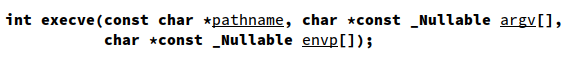
\includegraphics[width=0.7\textwidth]{execve_sig}
		\end{figure}

		که در آن
		\LRE{\verb|pathname|}
		آدرس فایل اجرایی برنامه (یا آدرس یک اسکریپت که با \LRE{shebang} آغاز می‌شود)،
		\LRE{\verb|argv|}
		آرگومان‌های خط‌فرمان برنامه، و
		\LRE{\verb|envp|}
		متغیرهای محیطی (
		\LRE{Environment variables})
		برنامه هستند.

		در اولین خط خروجی
		\LRE{strace}
		نیز می‌بینیم که این ابزار، با استفاده از همین سیستم‌کال، برنامه ما را اجرا کرده است؛ همچنین هیچ آرگومان خط‌فرمانی پاس داده نشده، و ۴۱ متغیر محیطی نیز به برنامه داده شده است.


		\item{
			\LRE{\verb|brk|}:
		}
		این سیستم‌کال، آدرس انتهای
		\LRE{Data Segment}
		پروسه (قسمتی از حافظه پروسه که شامل متغیر‌های
		\LRE{global}
		و
		\LRE{static}
		است) را تغییر می‌دهد. به این آدرس،
		\LRE{break}
		نیز گفته می‌شود. صدا‌زدن این سیستم‌کال با آدرس صفر، آدرس فعلی
		\LRE{break}
		را برمی‌گرداند و چیزی را تغییر نمی‌دهد.

		\item{
			\LRE{\verb|read|}:
		}
		از یک فایل، به مقدار مشخص شده داده می‌خواند و در یک بافر (فضایی در حافظه) می‌نویسد. امضای تابع مربوط به این سیستم‌کال در
		\LRE{glibc}
		به صورت زیر است؛

		\begin{figure}[H]
			\centering
			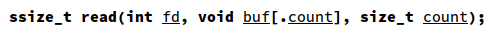
\includegraphics[width=0.6\textwidth]{read_sig}
		\end{figure}

		که در آن
		\LRE{\verb|fd|}
		شماره
		\LRE{file descriptor}
		مربوط به یک فایل باز شده توسط این پروسه،
		\LRE{\verb|buf|}
		آدرس بافر، و
		\LRE{\verb|count|}
		تعداد بایت‌هایی است که می‌خواهیم از فایل بخوانیم. در صورت موفقیت، این تابع علاوه بر نوشتن در بافر، تعداد بایت‌های خوانده شده را نیز برمی‌گرداند.

		\item{
			\LRE{\verb|write|}:
		}
		از یک بافر در حافظه، به مقدار مشخص شده داده می‌خواند و در یک فایل می‌نویسد. امضای تابع مربوط به این سیستم‌کال در
		\LRE{glibc}
		به شکل زیر است؛ که بسیار مشابه سیستم‌کال
		\LRE{\verb|read|}
		است.

		\begin{figure}[H]
			\centering
			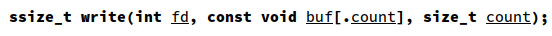
\includegraphics[width=0.65\textwidth]{write_sig}
		\end{figure}

		در خروجی
		\LRE{strace}
		مشاهده می‌کنیم که متن
		\LRE{\verb|"Hello world!"|}
		در فایلی با
		\LRE{file descriptor}
		برابر ۱ نوشته می‌شود و در نتیجه آن، این متن در خروجی استاندارد چاپ می‌شود. در لینوکس،
		\LRE{file descriptor}
		شماره ۱ همواره مربوط به خروجی استاندارد (یا
		\LRE{stdout})
		است، و در واقع با نوشتن در این فایل می‌توان متن را در خروجی چاپ کرد.
		(همچنین
		\LRE{fd}
		شماره صفر و ۲ نیز به ترتیب مربوط به
		\LRE{stdin}
		و
		\LRE{stderr}
		هستند.)

		\item{
			\LRE{\verb|close|}:
		}
		یک فایل باز را می‌بندد. تنها پارامتر آن نیز
		\LRE{fd}
		فایل مربوطه است.
	\end{itemize}

	\section*{سوال ۸}
	\paragraph*{}

	در مباحثه معروف بین
	\LRE{Torvalds}
	و
	\LRE{AST}
	به بسیاری از این دلایل اشاره شده است.
	\LRE{AST}
	معتقد بود که معماری
	\LRE{monolithic}
	منسوخ شده و متعلق به گذشته است، و معماری
	\LRE{micro-kernel}
	آینده معماری سیستم‌عامل‌ها است. خود او نیز سیستم‌عامل
	\LRE{Minix}
	را به عنوان یک سیستم‌عامل با قابلیت اجرا روی پردازنده‌های ارزان‌قیمت‌تر آن دوران و با اهداف آموزشی طراحی کرد که با معماری
	\LRE{micro-kernel}
	طراحی شده بود.
	\paragraph*{}
	در مقابل،
	\LRE{Torvalds}
	لینوکس را برای اجرا روی پردازنده
	\LRE{80386}
	اینتل و با معماری
	\LRE{monolithic}
	طراحی کرده بود. این پردازنده، نسبتا جدید و گران‌قیمت بود و حتی برای خود
	\LRE{Torvalds}
	هم مدتی طول کشید تا بتواند یکی از این پردازنده‌ها را برای خودش تهیه کند.

	\paragraph*{}
	\LRE{AST}
	دو اشکال عمده به لینوکس وارد می‌کرد، و به نظر او به همین دو دلیل کافی بود تا لینوکس «منسوخ‌شده» باشد:

	\begin{enumerate}
		\item {معماری
			\LRE{monolithic}:
		}
		\LRE{AST}
		طرفدار
		\LRE{micro-kernel}
		بود و این معماری لینوکس را بازگشتی به دهه ۷۰ میلادی می‌دانست.

		\item{
			\LRE{Portable}
			نبودن:
		}
		از دید
		\LRE{AST}،
		معماری پردازنده‌ها به سرعت در حال تغییر و تحول بودند و حتی پیش‌بینی می‌کرد که سری
		\LRE{80x86}
		اینتل کنار خواهد رفت و معماری‌های دیگر جایگزین آن خواهند شد؛ در نتیجه او طراحی سیستم‌عامل برای یک معماری خاص، به خصوص معماری عجیب و غریبی مثل
		\LRE{80x86}
		را اشتباه می‌دانست. او
		\LRE{Portability}
		را مهم می‌دانست و لینوکس را برای استفاده از قابلیت‌های خاص سخت‌افزاری
		\LRE{80386}
		که الزاما روی معماری‌های دیگر موجود نیست سرزنش می‌کرد، و معتقد بود به همین دلیل لینوکس به زودی فراموش خواهد شد.

		(به نظر می‌رسد پیش‌بینی او زیاد درست از آب در نیامده باشد...!)
	\end{enumerate}

	\paragraph*{}
	برخی پاسخ‌های
	\LRE{Torvalds}
	به این انتقادات، چنین بود:

	\begin{enumerate}
		\item
		او معماری
		\LRE{micro-kernel}
		را در مواردی مثل همروندی دچار مشکل می‌دانست؛ مثلا در حالی که لینوکس قابلیت
		\LRE{Multithreaded Filesystem}
		داشت و امکان کار با چندین فایل به طور همزمان را فراهم می‌کرد، در
		\LRE{minix}
		چنین قابلیتی موجود نبود.

		\item
		او معتقد بود که
		\LRE{micro-kernel}
		در نهایت کار طراحی سیستم‌عامل را پیچیده‌تر می‌کند و همان ارتباط مستقیم اجزای سیستم‌عامل با هم در یک کرنل
		\LRE{monolithic}
		سادگی بیشتری در طراحی دارد.

		\item
		از دید
		\LRE{Torvalds}،
		یک سیستم‌عامل نباید بیش از حد به
		\LRE{Portablity}
		اهمیت بدهد. چون سیستم‌عامل در نهایت لایه‌ای سطح‌بالاتر از سخت‌افزار است و مستقیم با سخت‌افزار ارتباط دارد و منطقی است که تا حدی از امکانات ویژه معماری‌های مختلف بهره ببرد.


	\end{enumerate}


	\paragraph*{}


\end{document}